\baitracnghiem{De01TNKQ:01}{
	Trong không gian $Oxyz$, hình chiếu vuông góc của điểm $M(-2;0;1)$ lên trục $Oy$ có tọa độ là:
}{
	\bonpa{1}
	{$(0;0;0)$.}
	{$(-2;0;0)$.}
	{$(-2;0;1)$.}
	{$(0;0;1)$;}
}{
	
}

\baitracnghiem{De01TNKQ:02}{
	Hàm số nào dưới đây luôn nghịch biến trên $\mathbb{R}$?
}{
	\bonpa{3}
	{$y=\frac{x^{2}+x+3}{x+2}$.}
	{$y=\frac{2x-2}{x+1}$.}
	{$y=3-2x-x^{3}$.}
	{$y=x^{3}+x+1$.}
}{
	
}

\baitracnghiem{De01TNKQ:03}{
	Cho hình hộp $ABCD.A'B'C'D'$. Tìm véc tơ $\overrightarrow{u}=\overrightarrow{AB}+\overrightarrow{AD}+\overrightarrow{CC'}$.
}{
	\bonpa{2}
	{$\overrightarrow{u}=\overrightarrow{AC}$.}
	{$\overrightarrow{u}=\overrightarrow{AC'}$.}
	{$\overrightarrow{u}=\overrightarrow{A'C}$.}
	{$\overrightarrow{u}=\overrightarrow{C'A}$.}
}{
	
}

\baitracnghiem{De01TNKQ:04}{
	Tìm điểm cực tiểu của đồ thị hàm số $y=\frac{1}{3}x^{3}-2x^{2}+3x+1$.
}{
	\bonpa{2}
	{$x=1$.}
	{$\left(1;\frac{7}{3}\right)$.}
	{$x=3$.}
	{$(3;1)$.}
}{
	
}

\baitracnghiem{De01TNKQ:05}{
	Cho hàm số $y=f(x)$ có bảng biến thiên như hình dưới. 
	
	\centerline{
		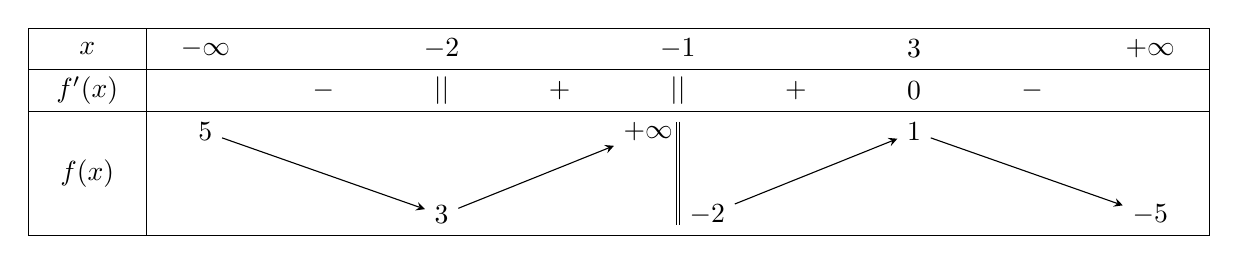
\begin{tikzpicture}[x=1.5cm,y=1.5em]
			\foreach \x/\gt in {0/x,1/-\infty,3/-2,5/-1,7/3,9/+\infty}\path (\x,0) node{$\gt$};
			\foreach \x/\gt in {0/f'(x),2/-,3/||,4/+,5/||,6/+,7/0,8/-}\path (\x,-1) node{$\gt$};
			\foreach \x/\y/\gt[count=\i from 0] in {0/-3/f(x),1/-2/5,3/-4/3,4.75/-2/+\infty,5.25/-4/-2,7/-2/1,9/-4/-5}\path (\x,\y) node(\i){$\gt$};
			\foreach \x/\y in {1/2,2/3,4/5,5/6}\draw[-stealth] (\x)--(\y);
			\draw (-.5,.5) rectangle (9.5,-4.5) (.5,.5)--(.5,-4.5) (-.5,-.5)--(9.5,-.5) (-.5,-1.5)--(9.5,-1.5);
			\draw[double] (5,-1.75)--(5,-4.25);
		\end{tikzpicture}
	}
	
	Đồ thị hàm số đã cho có tiệm cận đứng là:
}{
	\bonpa{1}
	{$x=-1$.}
	{$x=-2$.}
	{$y=1$.}
	{$y=5$.}
}{
	
}

\baitracnghiem{De01TNKQ:06}{
	Đường cong trong hình dưới đây là đồ thị của hàm số nào?
	
	\centerline{
		\begin{tikzpicture}
			\draw[-stealth] (-3,0)--(2,0) node[below]{$x$};
			\draw[-stealth] (0,-2.5)--(0,3) node[left]{$y$};
			\clip (-3,-2.5) rectangle (3,2);
			\draw[dashed] (-2,0) node[below]{$-2$}|-(0,2) node[right]{$2$};
			\draw[smooth] plot[domain=-3:3] (\x,{(\x)^3+3*(\x)^2-2});
			\path 
			(0,0) node[above left]{$O$}
			(-1,0) node[below]{$-1$}
			(0,-2) node[left]{$-2$}
			;
		\end{tikzpicture}
	}
	
}{
	\bonpa{2}
	{$y=-x^{3}-3x^{2}-2$.}
	{$y=x^{3}+3x^{2}-2$.}
	{$y=x^{3}-3x^{2}-2$.}
	{$y=-x^{3}+3x^{2}-2$.}
}{
	
}

\baitracnghiem{$De01TNKQ:07$}{
	Đường thẳng $x=-1$ là tiệm cận đứng của hàm số nào sau đây?
}{
	\bonpa{3}
	{$y=\frac{x+1}{x^{2}+4x+3}$.}
	{$y=\frac{x+1}{x^{2}+1}$.}
	{$y=\frac{x^{2}-3x+2}{x^{2}-1}$.}
	{$y=\frac{x^{2}+3x+2}{x^{2}-1}$.}
}{
	
}

\baitracnghiem{De01TNKQ:08}{
	Giá trị lớn nhất của hàm số $f(x)=\frac{3x-1}{x-3}$ trên $[0;2]$ là:
}{
	\bonpa{2}
	{$M=5$.}
	{$M=\frac{1}{3}$.}
	{$M=-5$.}
	{$M=-\frac{1}{3}$.}
}{
	
}

\baitracnghiem{De01TNKQ:09}{
	Gọi $A$ là giao điểm của đồ thị hàm số $y=\frac{x-2}{2x+1}$ với trục $Ox$. Giá trị đạo hàm của hàm số đã cho tại điểm $A$ là:
}{
	\bonpa{4}
	{$-\frac{5}{9}$.}
	{$-\frac{1}{3}$.}
	{$\frac{5}{9}$.}
	{$\frac{1}{3}$.}
}{
	
}

\baitracnghiem{De01TNKQ:10}{
	Cho lăng trụ đều $ABC.A'B'C'$. Góc giữa $\overrightarrow{BA}$ và $\overrightarrow{C'B'}$ bằng:
}{
	\bonpa{3}
	{$30^{\circ}$.}
	{$60^{\circ}$.}
	{$120^{\circ}$.}
	{$90^{\circ}$.}
}{
	
}

\baitracnghiem{De01TNKQ:11}{
	Trong không gian $Oxyz$. Cho điểm $M$ thỏa mãn $\overrightarrow{OM}=2\overrightarrow{i}-\overrightarrow{k}$. Khi đó tọa độ của điểm $M$ là:
}{
	\bonpa{2}
	{$(2;-1;0)$.}
	{$(2;0;-1)$.}
	{$(0;2;-1)$.}
	{$(-2;0;1)$.}
}{
	
}

\baitracnghiem{De01TNKQ:12}{
	Hàm số $f(x)=x^{3}-3x^{2}+1$ đạt cực đại tại:
}{
	\bonpa{4}
	{$x=2$.}
	{$y=2$.}
	{$y=0$.}
	{$x=0$.}
}{
	
}

\baitracnghiem{De01TNKQ:13}{
	Cho hàm số $f(x)$ có bảng biến thiên như sau:
	
	\centerline{
		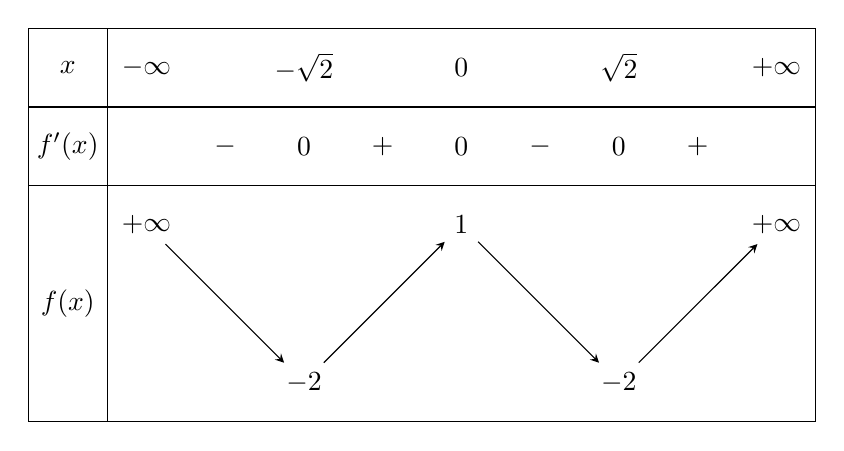
\begin{tikzpicture}
			\foreach \x/\gt in {0/x,1/-\infty,3/-\sqrt{2},5/0,7/\sqrt{2},9/+\infty}\path (\x,0) node{$\gt$};
			\foreach \x/\gt in {0/f'(x),2/-,3/0,4/+,5/0,6/-,7/0,8/+}\path (\x,-1) node{$\gt$};
			\foreach \x/\y/\gt[count=\i from 0] in {0/-3/f(x),1/-2/+\infty,3/-4/-2,5/-2/1,7/-4/-2,9/-2/+\infty}\path (\x,\y) node(\i){$\gt$};
			\foreach \x/\y in {1/2,2/3,3/4,4/5}\draw[-stealth] (\x)--(\y);
			\draw (-.5,.5) rectangle (9.5,-4.5) (.5,.5)--(.5,-4.5) (-.5,-.5)--(9.5,-.5) (-.5,-1.5)--(9.5,-1.5); 
		\end{tikzpicture}
	}
	
	Hàm số $f(x)$ nghịch biến trên khoảng nào?
}{
	\bonpa{2}
	{$(-\sqrt{2};\sqrt{2})$.}
	{$(-\infty;-\sqrt{2})$.}
	{$(-\sqrt{2};0)$.}
	{$(\sqrt{2};+\infty)$.}
}{
	
}

\baitracnghiem{De01TNKQ:14}{
	Hàm số $f(x)=\sqrt{x^{2}-2x}$ nghịch biến trên khoảng nào sau đây?
}{
	\bonpa{3}
	{$(2;+\infty)$.}
	{$(0,2)$.}
	{$(-\infty;0)$.}
	{$\mathbb{R}$.}
}{
	
}
%%10:59:48 10/11/2024Last Modification of contents